%%%%%%%%%%%%%%%%%%%%%%%%%%%%%%%%%%%%%%%%%%%%%%%%%%%%%%
% A Beamer template for HKUST (GZ)                   %
% Based on THU beamer theme                          %
% Author: Yuxuan HU                                  %
% Date: Aug 2024                                    %
% LPPL Licensed.                                     %
%%%%%%%%%%%%%%%%%%%%%%%%%%%%%%%%%%%%%%%%%%%%%%%%%%%%%%

\documentclass[serif, aspectratio=169]{beamer}
%\documentclass[serif]{beamer}  % for 4:3 ratio
\usepackage[T1]{fontenc} 
\usepackage{fourier} % see "http://faq.ktug.org/wiki/uploads/MathFonts.pdf" for other options
\usepackage{hyperref}
\usepackage{algorithm}
\usepackage{algpseudocode}
\usepackage{amsmath}
\usepackage{physics}
\usepackage{latexsym,amsmath,xcolor,multicol,booktabs,calligra}
\usepackage{graphicx,pstricks,listings,stackengine}

% usepackage for bibliography
\usepackage[backend=biber,style=authoryear]{biblatex}
\addbibresource{references.bib}

\author{Nihar Shah}
\title{Hybrid quantum-classical algorithms for solving eigenvalue problems}
\subtitle{}
\institute{
   @niharmayur@iisc.ac.in \\
    Department of Computational and Data Sciences \\
    Indian Institute of Science \\
}
\date{\small \today}
\usepackage{HKUSTstyle}

% defs
\def\cmd#1{\texttt{\color{red}\footnotesize $\backslash$#1}}
\def\env#1{\texttt{\color{blue}\footnotesize #1}}
% set colors
\definecolor{hkustyellow}{RGB}{167, 131, 55}
\definecolor{hkustblue}{RGB}{0, 56, 116}
\definecolor{hkustred}{RGB}{209, 51, 59}


\lstset{
    basicstyle=\ttfamily\small,
    keywordstyle=\bfseries\color{deepblue},
    emphstyle=\ttfamily\color{deepred},    % Custom highlighting style
    stringstyle=\color{deepgreen},
    numbers=left,
    numberstyle=\small\color{halfgray},
    rulesepcolor=\color{red!20!green!20!blue!20},
    frame=shadowbox,
}
%- --- --- --- --- --- --- --- --- --- --- --- --- --- --- --- 

\begin{document}

\begin{frame}
    \titlepage
    \vspace*{-0.6cm}
    \begin{figure}[htpb]
        \begin{center}
            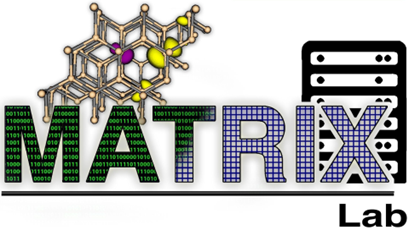
\includegraphics[keepaspectratio, scale=0.5]{pic/matrixlab.png}
        \end{center}
    \end{figure}
\end{frame}

\begin{frame}    
\tableofcontents[sectionstyle=show,
subsectionstyle=show/shaded/hide,
subsubsectionstyle=show/shaded/hide]
\end{frame}

% Introduction --- --- --- --- --- --- --- --- --- --- --- --- 
\section{The Problem}
\begin{frame}{To Find $n$ Smallest Eigenvalues}
    \frametitle<presentation>{To Find $n$ Smallest Eigenvalues}
        \begin{block}{
            \[
            \left(-\frac{1}{2}\nabla^2 + V(x)\right)\psi_I(x) = \lambda_I \psi_I(x)
            \]}
        \end{block}
    \begin{block}{Assumptions}
        \begin{itemize}
            \item Finite Difference Method (FDM) using a $2^{\text{nd}}$ order accurate Central Difference Scheme for Laplacian.
            \item Uniform grid: $\Delta x = \Delta y = \Delta z$.
            \item One-Dimensional problem.
        \end{itemize}
    \end{block}
\end{frame}

\begin{frame}{Discretized Equation}
    \[
    \begin{bmatrix}
        \ddots & \ddots & 0 & \ldots & 0 \\
        \ddots & \ddots & \ddots & \ldots & \vdots \\
        0 & -\frac{1}{2} & 1+V(x) & -\frac{1}{2} & 0 \\
        \vdots & \ldots & \ddots & \ddots &\ddots  \\
        0 & \ldots & 0 & \ddots & \ddots 
    \end{bmatrix}
    \begin{bmatrix}
        \vdots \\
        \psi(x_i - \Delta x)\\
        \psi(x_i)\\
        \psi(x_i + \Delta x)\\
        \vdots \\
    \end{bmatrix}
    =\lambda \begin{bmatrix}
        \vdots \\
        \psi(x_i-\Delta x)\\
        \psi(x_i)\\
        \psi(x_i+\Delta x) \\
        \vdots
    \end{bmatrix}
    \]
    \[
    \mathbf{H \psi}=\lambda\mathbf{\psi}
    \]
    where $\mathbf{H}$ is a Real Symmetric (Tridiagonal) Matrix.
\end{frame}

\begin{frame}{Popular Subspace Iteration (SI) Methods}
    
    \begin{table}
        \centering
        \begin{tabular}{|c|c|}
        % \hline
            Krylov Subspace Iteration Method & Chebyshev Subspace Iteration Method\\
            \hline
            Fast & Slower\\
            % \hline
            Optimal in a certain sense & Geared towards subspaces (vs individual eigenvalues) \\
            % \hline
            Requires one starting vector & \\
            % \hline
            Not easy to update & Updates are Easy \\
            % \hline
            Changes in $\mathbf{H}$ not allowed & Tolerates changes in $\mathbf{H}$ \\
            % \hline
        \end{tabular}
        \caption{Comparison between Krylov and Chebyshev subspace iteration method}
        \label{tab:comp}
    \end{table}
\end{frame}

\section{The Proposal}
\begin{frame}{Quantum Chebyshev Filtered Subspace Iteration (ChFSI) Algorithm (Part 1)}
    \begin{algorithm}[H]
        \caption{Quantum Chebyshev Filtered Subspace Iteration (ChFSI) Algorithm}
        \begin{algorithmic}[1]
            \State \textbf{Input:} Matrix $\mathbf{H}$, initial guess $\boldsymbol{\Psi_0}^{(0)} \in \mathbb{C}^{M\times N}$, Chebyshev polynomial degree $k$, subspace size $N (N > \tilde{N})$.
            \State \textbf{Output:} $n$ smallest eigenvalues and corresponding eigenvectors.
            \State \textbf{For iterations $t=0,1,2,\ldots,\max_{1\leq i\leq n} |\tilde{\lambda_i}^{(t)} - \tilde{\lambda_i} ^{(t)} |\leq\epsilon$} (\textbf{Convergence Criteria}) 
            \State \hspace{1em} \textbf{Chebyshev Filtering:} 
            \[
            \boldsymbol{\Psi_F}^{(t)} = T_k (\mathbf{H})\boldsymbol{\Psi_{0}}^{(t)}
            \]
            \hspace{1em} where $T_k$ is the Chebyshev polynomial of degree $k$ of the first kind.
            \State \hspace{1em} \textbf{Rayleigh-Ritz Projection:}
            \newline
            \hspace{1em} Compute Projected entries:
            \[
            \mathbf{\tilde{H}} = \boldsymbol{\Psi_F^{(t)\dagger}}\mathbf{H}\boldsymbol{\Psi_F^{(t)}}
            \]
        \end{algorithmic}
    \end{algorithm}
\end{frame}

\begin{frame}{Quantum Chebyshev Filtered Subspace Iteration (ChFSI) Algorithm (Part 2)}
    \begin{algorithm}[H]
        \begin{algorithmic}[1]
            \State \hspace{1em} Compute Overlap Matrix:
            \[
            \mathbf{\tilde{S}}=\boldsymbol{\Psi_F}^{(t)\dagger} \boldsymbol{\Psi_F}^{(t)}
            \]
            \State \hspace{1em} \textbf{Eigen-decomposition:} (on a classical computer)  
            \[
            \mathbf{\tilde{H}}\mathbf{Q}^{(t)}=\mathbf{\tilde{S}}\mathbf{Q}^{(t)}\boldsymbol{\tilde{\Lambda}}^{(t)}
            \]
            \State \hspace{1em} \textbf{Quantum Subspace rotation:}
            \[
            \boldsymbol{\Psi_0}^{(t+1)}=\boldsymbol{\Psi_F}^{(t)}\mathbf{Q}^{(t)}
            \]
        \end{algorithmic}
    \end{algorithm}
\end{frame}

\begin{frame}{Details}
    Given Eigenvalue Problem ($n$ smallest eigenvalues):
    \[
    \mathbf{HX}=\boldsymbol{\Lambda} \mathbf{X}
    \]
    where $\mathbf{X} \in \mathbb{C}^{m\times m},\mathbf{H}\in\mathbb{C}^{m\times m},\boldsymbol{\Lambda}\in\mathbb{C}^{m\times m}$
    \begin{itemize}
        \item Initial guess with $1$ random vector $\ket{\psi_0}$ (instead of $n$ random vectors):
        \[
        \boldsymbol{\Psi_0}^{(0)}=\begin{bmatrix}
            \vdots & \vdots & \ldots & \vdots \\
            \ket{\psi_0} & T_1(\mathbf{H})\ket{\psi_0} & \ldots & T_{n-1}(\mathbf{H})\ket{\psi_0}\\
            \vdots & \vdots & \ldots & \vdots 
        \end{bmatrix}
        \]
        We define $i^{th}$ column of $\boldsymbol{\Psi_0}^{(t)}$ as $\ket{\psi_i^{(t)}}$. Here, $\ket{\psi_i^{(0)}}=T_i(\mathbf{H})\ket{\psi_0}$; $\forall i=0,\ldots,n-1$.
    \end{itemize}
\end{frame}
\begin{frame}{Continued}
    For iterations $t=01,2,\ldots,\text{till convergence}$.
    \begin{itemize}
        \item \textbf{Chebyshev Filtering:}
        \begin{align*}
        \boldsymbol{\Psi_F}^{(t)}=T_k (\mathbf{H})\boldsymbol{\Psi_0}^{(t)}& = \begin{bmatrix}
            \vdots & \vdots & \ldots & \vdots \\
            T_k(\mathbf{H})\ket{\psi_0} & T_k(\mathbf{H})T_1(\mathbf{H})\ket{\psi_0} & \ldots & T_k(\mathbf{H})T_{n-1}(\mathbf{H})\ket{\psi_0} \\
            \vdots & \vdots & \ldots & \vdots
        \end{bmatrix}\\
        &=\begin{bmatrix}
        \vdots & \vdots & \ldots & \vdots \\
        T_k(\mathbf{H})\ket{\psi_0^{(t)}} & T_k(\mathbf{H})\ket{\psi_1^{(t)}} & \ldots & T_k(\mathbf{H})\ket{\psi_{n-1}^{(t)}}\\
        \vdots & \vdots & \ldots & \vdots
        \end{bmatrix}
        \end{align*}
   \end{itemize}
\end{frame}

\begin{frame}{Rayleigh-Ritz Projection}
    \begin{itemize}
        \item To find entries of the projected entries $\tilde{\mathbf{H}}=\boldsymbol{\Psi_F}^{(t)\dagger}\mathbf{H}\boldsymbol{\Psi_F}^{(t)}$, which is
        \begin{itemize}
            \item $\tilde{H}_{ij}=\bra{\psi_i^{(t)}}T_k(\mathbf{H})\mathbf{H}T_k(\mathbf{H})\ket{\psi_j^{(t)}}$
            \item $\tilde{S}_{ij}=\bra{\psi_i^{(t)}}T_k(\mathbf{H})\mathbf{H}T_K(\mathbf{H})\ket{\psi_j^{(t)}}$
        \end{itemize}
        $\forall i,j=0,\ldots,n-1$
         \item Simplify using Property of Chebyshev Polynomials:
        \[
        T_i(x)T_j(x)=\frac{1}{2}\left(T_{i+j}(x)+T_{|i-j|}(x)\right)
        \]
        \item Matrix elements of $\tilde{\mathbf{H}}$ and $\tilde{\mathbf{S}}$ are linear combinations of the inner products.
        \[
        \tilde{H}_{ij}=\frac{1}{4}\left(\bra{\psi_i^{(t)}}T_{2k+1}(\mathbf{H})+2T_1(\mathbf{H})+T_{2k-1}(\mathbf{H})\ket{\psi_j^{(t)}}\right)
        \]
        \[
        \tilde{S}_{ij}=\frac{1}{2}\left(\bra{\psi_i^{(t)}}T_{2k+1}(\mathbf{H})+T_0(\mathbf{H})\ket{\psi_j^{(t)}}\right)
        \]
    \end{itemize}
\end{frame}

\begin{frame}
    \[
    \tilde{H}_{ij} = \frac{1}{4}\left(\bra{\psi_i^{(t)}}T_{2k+1}(\mathbf{H})\ket{\psi_j^{(t)}} + 2\bra{\psi_i^{(t)}}\mathbf{H}\ket{\psi_j^{(t)}} + \bra{\psi_i^{(t)}}T_{2k-1}(\mathbf{H})\ket{\psi_j^{(t)}}\right)
    \]
    \[
    \tilde{S}_{ij} = \frac{1}{2}\left( \bra{\psi_i^{(t)}}T_{2k+1}(\mathbf{H})\ket{\psi_j^{(t)}} + \bra{\psi_i^{(t)}}\ket{\psi_j^{(t)}}\right)
    \]
    $\forall i,j=0,\ldots,n-1$.
    Thus, we need to evaluate just the four inner products (can be done entirely parallel on a quantum computer) using \textbf{Amplitude Estimation Algorithm} as subroutine.
\end{frame}

\section{Block-encoding}
\begin{frame}
\small % or \footnotesize or \scriptsize
\begin{block}{Theorem: (Block-encoding of sparse-access matrices) ~\cite{Gily_n_2019}}
\end{block}
Let $\mathbf{H} \in \mathbb{C}^{M\times M}; M=2^m$ be a matrix that is $s_r$-row-sparse and $s_c$-column sparse, and each value of $\mathbf{H}$ has absolute value at most $1$. Suppose we have access to the following sparse access oracles acting on two $(m+1)$ qubit registers
\[
O_r:\ket{i}\ket{k}\rightarrow \ket{i}\ket{r_{ik}} \quad \forall i \in [M]-1,k\in[s_r] 
\]
\[
O_c:\ket{l}\ket{j}\rightarrow \ket{c_{lj}\ket{j}}\quad \forall l\in [s_c],j\in[M]-1,
\]
where $r_{ij}$ is the index for the $j$-th non-zero entry of the $i$-th row of $\mathbf{H}$,  or if there are less than $i$ nonzero entries than it is $j+2^m$, and similarly $c_{ij}$ is the index for the $i$-th non-zero entry  of the $j$-th column of $\mathbf{H}$, or if there are less than $j$ non zero entries, then it is $i+2^m$. Additionally assume that we have access to an oracle $O_A$ that returns the entries of $A$ in a binary description
    \[
    O_A:\ket{i}\ket{j}\ket{0}^{\otimes b}\rightarrow \ket{i}\ket{j}\ket{a_{ij}}\quad \forall i,j\in[M]-1
    \]
    where $a_{ij}$ is a $b$-bit binary description (for simplicity we assume here that the binary representation is exact) of the $ij$ matrix element of $A$. Then we can implement a $(\sqrt{s_rs_c},m+3,\epsilon)$ block-encoding of $A$ with a single use of $O_r$,$O_c$, two uses of $O_A$ and additionally using $O(m+\log^{2.5}\left(\frac{s_rs_c}{\epsilon}\right))$ one and two qubit gates while using $O(b,\log^{2.5}\left(\frac{s_rs_c}{\epsilon}\right))$ ancilla qubits.
\end{frame}

\begin{frame}
    \begin{itemize}
    \item Recall that $\mathbf{H}$ is a banded-s-sparse matrix. This can be encoded as Unitary $\mathbf{U_H}\in HBE(s,\lceil\log s\rceil,0)$
\end{itemize}
\end{frame}

\begin{frame}{References}
    \printbibliography
\end{frame}


\begin{frame}
\begin{center}
{ Thank you!}
\vspace{1cm}

Nihar Shah\\[1em]
`niharmayur@iisc.ac.in'
\end{center}
\end{frame}

\end{document}